\documentclass{standalone}
\usepackage{tikz}
\begin{document}
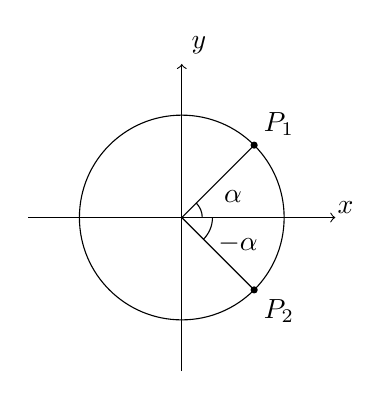
\begin{tikzpicture}[scale=1.3] 
\draw (0,0) circle (1cm);
\draw[->] (-1.5,0) -- (1.5,0);
\draw (1.6,0.1) node{$x$};
\draw[->] (0,-1.5) -- (0,1.5) node[anchor=south west] {$y$};
\draw (0,0) -- (0.707106781,0.707106781);
\draw (0,0) -- (0.707106781,-0.707106781);
\draw (0.2,0) arc(0:45:0.2);
\draw (0.3,0) arc(0:-45:0.3);
\draw (0.707106781,0.707106781) node[anchor=south west]{$P_1$};
\fill (0.707106781,0.707106781) circle(1pt);
\draw (0.707106781,-0.707106781) node[anchor=north west]{$P_2$};
\fill (0.707106781,-0.707106781) circle(1pt);
\draw  (0.5,0.2) node{$\alpha$};
\draw  (0.55,-0.25) node{$-\alpha$};

\end{tikzpicture}
\end{document}